\documentclass[aspectratio=169]{beamer}

% Theme and Color Setup
\usetheme{Madrid}
\usecolortheme{whale}
\useinnertheme{rectangles}
\useoutertheme{miniframes}

% Additional Packages
\usepackage[utf8]{inputenc}
\usepackage[T1]{fontenc}
\usepackage{graphicx}
\usepackage{booktabs}
\usepackage{listings}
\usepackage{amsmath}
\usepackage{amssymb}
\usepackage{xcolor}
\usepackage{tikz}
\usepackage{pgfplots}
\pgfplotsset{compat=1.18}
\usetikzlibrary{positioning}
\usepackage{hyperref}

% Custom Colors
\definecolor{myblue}{RGB}{31, 73, 125}
\definecolor{mygray}{RGB}{100, 100, 100}
\definecolor{mygreen}{RGB}{0, 128, 0}
\definecolor{myorange}{RGB}{230, 126, 34}
\definecolor{mycodebackground}{RGB}{245, 245, 245}

% Set Theme Colors
\setbeamercolor{structure}{fg=myblue}
\setbeamercolor{frametitle}{fg=white, bg=myblue}
\setbeamercolor{title}{fg=myblue}
\setbeamercolor{section in toc}{fg=myblue}
\setbeamercolor{item projected}{fg=white, bg=myblue}
\setbeamercolor{block title}{bg=myblue!20, fg=myblue}
\setbeamercolor{block body}{bg=myblue!10}
\setbeamercolor{alerted text}{fg=myorange}

% Set Fonts
\setbeamerfont{title}{size=\Large, series=\bfseries}
\setbeamerfont{frametitle}{size=\large, series=\bfseries}
\setbeamerfont{caption}{size=\small}
\setbeamerfont{footnote}{size=\tiny}

% Document Start
\begin{document}

\frame{\titlepage}

\begin{frame}[fragile]
    \title{Week 11: Data Ethics and Governance}
    \author{John Smith, Ph.D.}
    \date{\today}
    \maketitle
\end{frame}

\begin{frame}[fragile]
    \frametitle{Introduction to Data Ethics and Governance}
    \begin{block}{Overview of Ethical Data Practices}
        Data ethics refers to the moral principles that guide the collection, storage, sharing, and use of data. It emphasizes the importance of responsibility and accountability in how data is handled.
    \end{block}
    \begin{itemize}
        \item \textbf{Why is Data Governance Important?}
        \begin{itemize}
            \item Framework for managing data assets.
            \item Aligns data management strategies with ethical standards and legal requirements.
        \end{itemize}
    \end{itemize}
\end{frame}

\begin{frame}[fragile]
    \frametitle{The Intersection of Data Ethics and Governance}
    \begin{itemize}
        \item \textbf{Trust Building:} Ethical practices foster trust among stakeholders.
        \item \textbf{Compliance with Regulations:} Helps organizations comply with laws such as GDPR, HIPAA, etc.
        \item \textbf{Data Quality and Integrity:} Ensures accurate and trustworthy data for decision-making.
    \end{itemize}
\end{frame}

\begin{frame}[fragile]
    \frametitle{Key Concepts in Data Ethics}
    \begin{enumerate}
        \item \textbf{Transparency}
        \begin{itemize}
            \item Organizations should be clear about data handling practices.
            \item \textit{Example:} A social media platform discloses data usage for targeted advertising.
        \end{itemize}
        
        \item \textbf{Privacy}
        \begin{itemize}
            \item Protects individuals’ personal information.
            \item \textit{Example:} Implementing data encryption and privacy settings.
        \end{itemize}

        \item \textbf{Fairness}
        \begin{itemize}
            \item Prevents bias or discrimination against groups.
            \item \textit{Example:} Regularly auditing algorithms for bias against marginalized communities.
        \end{itemize}

        \item \textbf{Accountability}
        \begin{itemize}
            \item Establishes mechanisms for holding organizations responsible.
            \item \textit{Example:} Appointing a data ethics officer to oversee compliance.
        \end{itemize}
    \end{enumerate}
\end{frame}

\begin{frame}[fragile]
    \frametitle{Data Ethics Lifecycle}
    \begin{itemize}
        \item \textbf{Data Collection:} Fair and consensual practices.
        \item \textbf{Data Storage:} Prioritizing security and integrity.
        \item \textbf{Data Usage:} Ethical applications that prioritize user welfare.
        \item \textbf{Data Disposal:} Secure deletion to prevent data leaks.
    \end{itemize}
\end{frame}

\begin{frame}[fragile]
    \frametitle{Key Concepts in Data Ethics}
    \begin{itemize}
        \item Ethical principles governing data usage
        \item Importance of privacy, security, accountability, and fairness
    \end{itemize}
\end{frame}

\begin{frame}[fragile]
    \frametitle{Introduction to Data Ethics}
    \begin{block}{Definition}
        Data ethics refers to the moral principles guiding the collection, storage, processing, and dissemination of data.
    \end{block}
    \begin{itemize}
        \item Critical in today's data-driven world
        \item Focuses on issues related to privacy and security
    \end{itemize}
\end{frame}

\begin{frame}[fragile]
    \frametitle{1. Privacy}
    \begin{itemize}
        \item \textbf{Definition:} Right to control personal information
        \item \textbf{Key Principles:}
        \begin{itemize}
            \item Informed Consent: Awareness and agreement on data collection
            \item Data Minimization: Only collect necessary data
        \end{itemize}
        \item \textbf{Example:} User consent required before sharing on social media platforms
    \end{itemize}
\end{frame}

\begin{frame}[fragile]
    \frametitle{2. Security}
    \begin{itemize}
        \item \textbf{Definition:} Protective measures against unauthorized access
        \item \textbf{Key Principles:}
        \begin{itemize}
            \item Confidentiality: Only authorized access to data
            \item Integrity: Accuracy and reliability maintenance
        \end{itemize}
        \item \textbf{Example:} Use of encryption for electronic data protection
    \end{itemize}
\end{frame}

\begin{frame}[fragile]
    \frametitle{3. Accountability}
    \begin{itemize}
        \item \textbf{Definition:} Responsibility for data practices
        \item \textbf{Key Principles:}
        \begin{itemize}
            \item Transparency: Clear data usage policies
            \item Redress: Mechanisms for reporting problems
        \end{itemize}
        \item \textbf{Example:} Companies providing policy clarity on user data management
    \end{itemize}
\end{frame}

\begin{frame}[fragile]
    \frametitle{4. Fairness}
    \begin{itemize}
        \item \textbf{Definition:} Equitable and non-discriminatory data practices
        \item \textbf{Key Principles:}
        \begin{itemize}
            \item Bias Detection: Regular algorithm assessments
            \item Inclusivity: Diverse representation in data collection
        \end{itemize}
        \item \textbf{Example:} Auditing hiring algorithms to prevent demographic bias
    \end{itemize}
\end{frame}

\begin{frame}[fragile]
    \frametitle{Key Points to Emphasize}
    \begin{itemize}
        \item Ethical data practices protect individual rights
        \item Foster trust between organizations and stakeholders
        \item Understanding is vital for responsible data governance
    \end{itemize}
\end{frame}

\begin{frame}[fragile]
    \frametitle{Visual Representation}
    \begin{itemize}
        \item A flowchart showcasing the relationship between:
        \begin{itemize}
            \item Privacy
            \item Security
            \item Fairness
            \item Accountability
        \end{itemize}
    \end{itemize}
    
    \begin{center}
        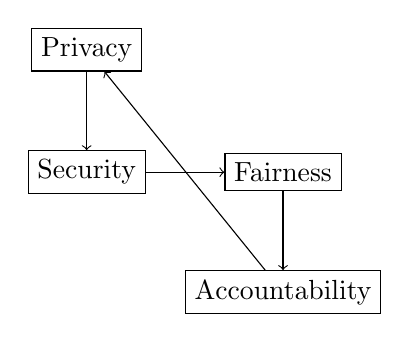
\begin{tikzpicture}
            \node (p) [draw, rectangle] {Privacy};
            \node (s) [draw, rectangle, below=of p] {Security};
            \node (f) [draw, rectangle, right=of s] {Fairness};
            \node (a) [draw, rectangle, below=of f] {Accountability};
            
            \draw[->] (p) -- (s);
            \draw[->] (s) -- (f);
            \draw[->] (f) -- (a);
            \draw[->] (a) -- (p);
        \end{tikzpicture}
    \end{center}
\end{frame}

\begin{frame}[fragile]
    \frametitle{Conclusion}
    \begin{itemize}
        \item Upholding ethical standards in data usage is essential
        \item Protect personal information and foster trust
        \item Adopt these principles for responsible data governance
    \end{itemize}
\end{frame}

\begin{frame}[fragile]
    \frametitle{Data Governance Frameworks}
    \begin{block}{Introduction}
        Data Governance refers to the overall management of the availability, usability, integrity, and security of data in an organization. 
        Data Governance Frameworks provide structured approaches to ensure that data is managed effectively and aligned with business goals.
    \end{block}
\end{frame}

\begin{frame}[fragile]
    \frametitle{Key Components of Data Governance Frameworks}
    \begin{enumerate}
        \item \textbf{Data Stewardship}
            \begin{itemize}
                \item Definition: Roles and responsibilities that oversee data assets.
                \item Example: Designating a data steward responsible for data quality standards.
            \end{itemize}
        \item \textbf{Data Quality Management}
            \begin{itemize}
                \item Definition: Processes ensuring accuracy, completeness, reliability, and consistency of data.
                \item Example: Implementing validation checks during data entry.
            \end{itemize}
        \item \textbf{Data Policies and Standards}
            \begin{itemize}
                \item Definition: Guidelines governing data use.
                \item Example: A policy dictating access to customer data.
            \end{itemize}
        \item \textbf{Data Lifecycle Management}
            \begin{itemize}
                \item Definition: Managing data across its lifecycle.
                \item Example: Archiving outdated records to comply with retention policies.
            \end{itemize}
        \item \textbf{Compliance and Risk Management}
            \begin{itemize}
                \item Definition: Adherence to legal and regulatory requirements.
                \item Example: Conducting audits for GDPR compliance.
            \end{itemize}
    \end{enumerate}
\end{frame}

\begin{frame}[fragile]
    \frametitle{Best Practices in Data Governance}
    \begin{itemize}
        \item \textbf{Establish Clear Objectives:} Define governance goals aligned with business needs.
        \item \textbf{Engage Stakeholders:} Involve various departments in governance activities.
        \item \textbf{Create a Data Governance Committee:} Form a team to oversee policies and procedures.
        \item \textbf{Utilize Technology:} Implement tools to automate governance processes.
        \item \textbf{Regularly Review Policies:} Ensure governance policies evolve with changing environments.
    \end{itemize}
\end{frame}

\begin{frame}[fragile]
    \frametitle{Diagram: Data Governance Framework Overview}
    \begin{center}
        \includegraphics[width=0.8\textwidth]{path_to_your_diagram} % Replace with actual diagram path
    \end{center}
\end{frame}

\begin{frame}[fragile]
    \frametitle{Key Points to Emphasize}
    \begin{itemize}
        \item \textbf{Value of Data:} Treat data as a valuable asset requiring careful governance.
        \item \textbf{Holistic Approach:} Address technical, organizational, and regulatory aspects comprehensively.
        \item \textbf{Continuous Improvement:} Governance must adapt to evolving data management challenges.
    \end{itemize}
\end{frame}

\begin{frame}[fragile]
    \frametitle{Case Study: Ethical Dilemmas in Data Usage}
    % Overview of Ethical Dilemmas in Data Usage
    \begin{block}{Overview}
        Data usage in today’s digital world often raises significant ethical questions. These dilemmas are critical to assess as organizations strive to balance data-driven decision-making with the responsibility to uphold ethical standards.
    \end{block}
\end{frame}

\begin{frame}[fragile]
    \frametitle{Key Ethical Issues in Data Usage}
    % Key Ethical Issues
    \begin{enumerate}
        \item \textbf{Informed Consent}
            \begin{itemize}
                \item Do users fully understand how their data will be used?
                \item Example: A social media platform updates its privacy policy, allowing the sale of user data without explicit consent.
            \end{itemize}
        \item \textbf{Data Privacy}
            \begin{itemize}
                \item Are individuals’ personal details sufficiently protected?
                \item Example: A healthcare provider experiences a data breach exposing patient records.
            \end{itemize}
        \item \textbf{Bias and Discrimination}
            \begin{itemize}
                \item Are algorithms creating unfair biases in decision-making processes?
                \item Example: A hiring algorithm disproportionately disqualifies candidates from certain demographic groups.
            \end{itemize}
        \item \textbf{Security}
            \begin{itemize}
                \item Is data adequately protected against unauthorized access?
                \item Example: A company faces backlash after failing to secure customer data, resulting in a major breach.
            \end{itemize}
        \item \textbf{Accountability}
            \begin{itemize}
                \item Who is held responsible for unethical data practices?
                \item Example: A financial institution misuses customer data for profit without accountability measures in place.
            \end{itemize}
    \end{enumerate}
\end{frame}

\begin{frame}[fragile]
    \frametitle{Case Study: Cambridge Analytica}
    % Cambridge Analytica Scandal
    \begin{block}{Background}
        Cambridge Analytica utilized data from Facebook users without their consent to develop psychological profiles for political advertising.
    \end{block}
    \begin{itemize}
        \item \textbf{Ethical Issues:}
            \begin{itemize}
                \item \textbf{Informed Consent:} Users were unaware their data was being harvested for political targeting.
                \item \textbf{Data Privacy:} Sensitive information was used without explicit permission.
                \item \textbf{Bias:} Targeted ads reinforced existing prejudices.
            \end{itemize}
        \item \textbf{Consequences:} 
            \begin{itemize}
                \item Legal actions against Facebook and Cambridge Analytica.
                \item Reforms in data governance and stricter regulations on data privacy.
            \end{itemize}
    \end{itemize}
\end{frame}

\begin{frame}[fragile]
    \frametitle{Key Points and Ethical Framework}
    % Key Points to Emphasize
    \begin{itemize}
        \item \textbf{Awareness:} Understanding ethical dilemmas helps organizations improve data governance practices.
        \item \textbf{Impact of Decisions:} Ethical missteps not only lead to legal repercussions but also damage brand reputation.
        \item \textbf{Best Practices:} Establish clear guidelines for data usage, guarantee informed consent, and regularly review data governance frameworks.
    \end{itemize}
    
    \begin{block}{Ethical Framework for Data Usage}
        \begin{enumerate}
            \item Identify Stakeholders
            \item Assess Risks and Impacts
            \item Implement Transparency and Consent
            \item Monitor and Evaluate Outcomes
            \item Adjust Policies and Practices
        \end{enumerate}
    \end{block}
\end{frame}

\begin{frame}[fragile]
    \frametitle{Evaluating Data Governance Strategies}
    \begin{block}{Introduction to Data Governance}
    Data governance is a framework for managing data availability, usability, integrity, and security across an organization. It involves the implementation of policies, procedures, and standards that ensure data is handled properly and ethically.
    \end{block}
\end{frame}

\begin{frame}[fragile]
    \frametitle{Key Concepts of Data Governance Strategies}
    \begin{itemize}
        \item \textbf{Data Stewardship:} Assigning data stewards responsible for overseeing data management practices, ensuring compliance with laws and regulations, and applying data governance policies.
        
        \item \textbf{Data Quality Management:} Establishing processes to ensure accuracy, consistency, and completeness of data throughout its lifecycle.
        
        \item \textbf{Compliance and Legal Framework:} Implementing strategies to adhere to relevant laws (like GDPR, HIPAA) regarding data privacy and security.
        
        \item \textbf{Metadata Management:} Maintaining a repository of metadata to track data lineage, definitions, and usage rules, enhancing transparency and understanding of data assets.
        
        \item \textbf{Risk Management:} Identifying and mitigating risks associated with data handling, including data breaches and misuse, through continuous monitoring and assessment.
    \end{itemize}
\end{frame}

\begin{frame}[fragile]
    \frametitle{Strategies for Effective Data Governance}
    \begin{enumerate}
        \item \textbf{Develop Clear Policies:}
            \begin{itemize}
                \item Create and document data governance policies that clarify roles, responsibilities, and standard practices.
                \item Example: An organization might establish a policy that prohibits sharing customer data with third parties without explicit consent.
            \end{itemize}
        
        \item \textbf{Engage Stakeholders:}
            \begin{itemize}
                \item Involve various stakeholders from different departments (IT, legal, compliance, business units) in the governance process for a well-rounded approach.
                \item Example: Form a cross-functional data governance committee that meets regularly to review policies and address concerns.
            \end{itemize}
        
        \item \textbf{Use Data Governance Frameworks:}   
        Adopt established frameworks like DAMA-DMBOK (Data Management Body of Knowledge) or DCAM (Data Management Capability Assessment Model) as guiding structures.
        
        \item \textbf{Implement Technology Solutions:}
            \begin{itemize}
                \item Utilize data governance tools and software (like Collibra, Alation) to automate data cataloging, lineage tracking, and compliance checks.
                \item Example: A data discovery tool can help identify sensitive data across various systems, ensuring it’s secured properly.
            \end{itemize}
        
        \item \textbf{Training and Awareness Programs:}
            \begin{itemize}
                \item Conduct training sessions for employees to raise awareness about data governance principles and their importance in the organization.
                \item Example: Offer workshops that explain data privacy laws and the organization's data use policies, emphasizing employee roles in compliance.
            \end{itemize}
    \end{enumerate}
\end{frame}

\begin{frame}[fragile]
    \frametitle{Key Points to Emphasize}
    \begin{itemize}
        \item Data governance is essential for maintaining the ethical use of data.
        \item A strong governance strategy can enhance data quality and integrity, leading to better decision-making.
        \item Continuous assessment and improvement of governance strategies are vital as business needs and regulations evolve.
    \end{itemize}
\end{frame}

\begin{frame}[fragile]
    \frametitle{Data Governance Framework}
    \begin{block}{Diagram: Data Governance Framework}
    \begin{verbatim}
    +-----------------------------------------------------+
    |            Data Governance Strategy                  |
    | +-------------------+ +-------------------------+    |
    | |    Policies &     | |   Compliance & Legal    |  |
    | |    Standards      | |      Frameworks         |  |
    | +-------------------+ +-------------------------+  |
    |            |                                              |
    | +-------------------+ +-------------------------+        |
    | |      Data         | |     Training &          |       |
    | |    Stewardship     | |     Awareness          |       |
    | +-------------------+ +-------------------------+        |
    |            |                                              |
    | +-------------------+ +-------------------------+        |
    | |   Technology &    | |     Risk Management      |       |
    | |   Automation      | |                         |       |
    | +-------------------+ +-------------------------+        |
    +-----------------------------------------------------+
    \end{verbatim}
    \end{block}
\end{frame}

\begin{frame}[fragile]
    \frametitle{Impact of Poor Data Governance}
    \begin{block}{Understanding Poor Data Governance}
        Poor data governance refers to a lack of effective policies, processes, and controls in managing data. This inadequacy can lead to numerous challenges for organizations and stakeholders involved.
    \end{block}
\end{frame}

\begin{frame}[fragile]
    \frametitle{Key Consequences of Inadequate Data Governance}
    \begin{enumerate}
        \item \textbf{Data Quality Issues}
            \begin{itemize}
                \item \textbf{Description:} Without proper governance, data can become inaccurate, incomplete, or inconsistent.
                \item \textbf{Example:} An e-commerce company mismanaging its product inventory data may present incorrect stock levels, leading to customer dissatisfaction.
            \end{itemize}

        \item \textbf{Compliance Risks}
            \begin{itemize}
                \item \textbf{Description:} Non-compliance with data protection regulations can result in legal actions and heavy fines.
                \item \textbf{Example:} A healthcare provider failing to secure patient data may face significant penalties for violating regulations.
            \end{itemize}

        \item \textbf{Loss of Trust}
            \begin{itemize}
                \item \textbf{Description:} Failure to manage data responsibly erodes trust in the organization.
                \item \textbf{Example:} A data breach can lead to customer distrust, prompting them to shift to competitors.
            \end{itemize}
    \end{enumerate}
\end{frame}

\begin{frame}[fragile]
    \frametitle{Key Consequences Continued}
    \begin{enumerate}[resume]
        \item \textbf{Inefficient Decision-Making}
            \begin{itemize}
                \item \textbf{Description:} Poor governance hampers access to reliable data, leading to uninformed decision-making.
                \item \textbf{Example:} A finance team using error-laden sales forecasts may make poor investment decisions.
            \end{itemize}
        
        \item \textbf{Increased Costs}
            \begin{itemize}
                \item \textbf{Description:} Inefficiencies from poor data management can lead to significant cost increases in remediation efforts.
                \item \textbf{Example:} Companies that spend excessive time correcting data inaccuracies lose resources and competitive advantage.
            \end{itemize}
    \end{enumerate}
    
    \pause
    \begin{block}{Key Points to Emphasize}
        \begin{itemize}
            \item Effective data governance ensures data quality, compliance, and organizational integrity.
            \item The costs of poor governance can severely impact bottom lines.
            \item Strong governance strategies mitigate risks and enhance decision-making capabilities.
        \end{itemize}
    \end{block}
\end{frame}

\begin{frame}[fragile]
    \frametitle{Data Governance Impact Flow Diagram}
    \begin{center}
        \includegraphics[width=0.8\textwidth]{data_governance_flow_diagram.png} % Placeholder for the diagram
    \end{center}
    \begin{block}{Flow Structure}
        Poor Data Governance $\rightarrow$ Data Quality Issues \\
                                        $\downarrow$ \\
                                        Compliance Risks $\rightarrow$ Loss of Trust \\
                                        $\downarrow$ \\
                                        Inefficient Decision-Making \\
                                        $\downarrow$ \\
                                        Increased Costs $\rightarrow$ Organizational Performance Impact
    \end{block}
\end{frame}

\begin{frame}[fragile]
    \frametitle{Summary}
    Understanding and addressing the impacts of poor data governance is essential for organizations looking to thrive in a data-driven environment. By implementing effective data governance strategies, organizations can safeguard their data assets, enhance credibility, and drive better decision-making practices.
\end{frame}

\begin{frame}[fragile]
    \frametitle{Role of Legislation in Data Ethics}
    \begin{itemize}
        \item Legislation shapes ethical standards for data management.
        \item Protects individual rights and ensures accountability.
        \item Focus on GDPR and other significant frameworks.
    \end{itemize}
\end{frame}

\begin{frame}[fragile]
    \frametitle{Key Legislation Affecting Data Ethics}
    \begin{enumerate}
        \item \textbf{General Data Protection Regulation (GDPR)}
            \begin{itemize}
                \item Enacted: May 25, 2018
                \item Purpose: Protect personal data and privacy of EU citizens.
                \item Key Principles:
                    \begin{itemize}
                        \item Data Minimization
                        \item Purpose Limitation
                        \item Consent
                        \item Right to Access
                    \end{itemize}
            \end{itemize}
        \item \textbf{California Consumer Privacy Act (CCPA)}
            \begin{itemize}
                \item Enacted: January 1, 2020
                \item Purpose: Enhance privacy rights for California residents.
                \item Key Features:
                    \begin{itemize}
                        \item Right to Know
                        \item Right to Delete
                        \item Opt-out Provision
                    \end{itemize}
            \end{itemize}
        \item \textbf{Health Insurance Portability and Accountability Act (HIPAA)}
            \begin{itemize}
                \item Enacted: 1996
                \item Purpose: Protect sensitive patient health information.
                \item Key Aspects:
                    \begin{itemize}
                        \item Privacy Rule
                        \item Security Rule
                    \end{itemize}
            \end{itemize}
    \end{enumerate}
\end{frame}

\begin{frame}[fragile]
    \frametitle{Importance of Data Legislation}
    \begin{itemize}
        \item \textbf{Trust Building:} 
            \begin{itemize}
                \item Fosters public trust in organizations managing personal data.
            \end{itemize}
        \item \textbf{Accountability:} 
            \begin{itemize}
                \item Penalties for non-compliance ensure adherence to ethical practices.
            \end{itemize}
        \item \textbf{Global Standards:} 
            \begin{itemize}
                \item GDPR serves as a benchmark for data protection worldwide.
            \end{itemize}
    \end{itemize}
\end{frame}

\begin{frame}[fragile]
    \frametitle{Key Points to Emphasize}
    \begin{itemize}
        \item Legislation like GDPR and CCPA enhances control over personal data.
        \item Ethical data governance is a moral responsibility for organizations.
        \item Non-compliance can lead to financial penalties and reputational damage.
    \end{itemize}
\end{frame}

\begin{frame}[fragile]
    \frametitle{Visual Aid: Data Protection Framework}
    \begin{center}
        \texttt{
        [Data Protection Framework] \\
        +-------------------------+ \\
        |          GDPR          | \\
        |   +---------------+     | \\
        |   |    CCPA      |     | \\
        |   +---------------+     | \\
        |   |     HIPAA    |     | \\
        |   +---------------+     | \\
        +-------------------------+
        }
    \end{center}
    \textbf{Note:} This diagram shows how GDPR supports a comprehensive data protection framework complemented by CCPA and HIPAA.
\end{frame}

\begin{frame}[fragile]
    \frametitle{Conclusion}
    \begin{itemize}
        \item Understanding legislation's role in data ethics is critical.
        \item Laws guide ethical practices and ensure accountability.
        \item Consider these frameworks in upcoming discussions on ethical data handling.
    \end{itemize}
\end{frame}

\begin{frame}[fragile]
    \frametitle{Best Practices for Ethical Data Handling}
    \begin{block}{Introduction}
        The collection and use of data come with significant ethical responsibilities. It is crucial for organizations to establish practices that prioritize the rights and privacy of individuals.
    \end{block}
    This presentation outlines best practices that guide data practitioners towards responsible and ethical data handling.
\end{frame}

\begin{frame}[fragile]
    \frametitle{Key Best Practices - Part 1}
    \begin{enumerate}
        \item \textbf{Informed Consent}
            \begin{itemize}
                \item Obtain explicit permission before collecting data.
                \item Clearly explain the data's usage, storage, and sharing.
                \item Example: A healthcare provider informing patients about research use of their medical data.
            \end{itemize}
        \item \textbf{Data Minimization}
            \begin{itemize}
                \item Collect only necessary data for specific purposes.
                \item Avoid excessive data collection irrelevant to objectives.
                \item Example: An app requesting GPS location only if relevant to service delivery.
            \end{itemize}
    \end{enumerate}
\end{frame}

\begin{frame}[fragile]
    \frametitle{Key Best Practices - Part 2}
    \begin{enumerate}
        \setcounter{enumi}{2}
        \item \textbf{Anonymization and Pseudonymization}
            \begin{itemize}
                \item Remove or encrypt personally identifiable information (PII).
                \item Example: Replacing names with unique identification numbers.
            \end{itemize}
        \item \textbf{Transparency}
            \begin{itemize}
                \item Be open about data practices and provide clear information.
                \item Example: A concise privacy policy page detailing user data usage.
            \end{itemize}
        \item \textbf{Security Measures}
            \begin{itemize}
                \item Implement robust security protocols.
                \item Example: Utilizing two-factor authentication for sensitive accounts.
            \end{itemize}
    \end{enumerate}
\end{frame}

\begin{frame}[fragile]
    \frametitle{Key Best Practices - Part 3}
    \begin{enumerate}
        \setcounter{enumi}{5}
        \item \textbf{Regular Audits and Compliance}
            \begin{itemize}
                \item Conduct audits to ensure ethical standards and legal compliance.
                \item Example: Quarterly reviews of data collection practices.
            \end{itemize}
        \item \textbf{Training and Awareness}
            \begin{itemize}
                \item Provide ongoing training on data ethics and privacy regulations.
                \item Example: Regular workshops on data ethics for all employees.
            \end{itemize}
    \end{enumerate}
\end{frame}

\begin{frame}[fragile]
    \frametitle{Conclusion and Key Takeaway}
    Adopting these best practices safeguards individual privacy and builds trust with users and stakeholders. 
    \begin{block}{Key Takeaway}
        The ethical handling of data is not just a legal requirement, but a cornerstone of responsible data management that fosters trust and accountability.
    \end{block}
    Implementing these practices significantly impacts user confidence and organizational integrity.
\end{frame}

\begin{frame}[fragile]
    \frametitle{Group Discussion on Ethical Scenarios}
    
    \begin{block}{Introduction to Ethical Dilemmas in Data Governance}
        In today's data-driven world, ethical considerations play a pivotal role in how organizations manage data. Ethical dilemmas arise when there are conflicts between data utility and the ethical treatment of individuals whose data is being processed. This discussion focuses on engaging with hypothetical scenarios to critically assess our understanding of data ethics and governance.
    \end{block}
\end{frame}

\begin{frame}[fragile]
    \frametitle{Key Concepts in Data Ethics}

    \begin{enumerate}
        \item \textbf{Data Governance}:
        \begin{itemize}
            \item Refers to the policies, procedures, and standards that dictate how data is managed and used within an organization.
            \item Ensures data integrity, availability, and confidentiality.
        \end{itemize}

        \item \textbf{Data Ethics}:
        \begin{itemize}
            \item Involves the moral obligations regarding how data should be collected, stored, utilized, and shared.
            \item Encompasses principles such as consent, transparency, accountability, and fairness.
        \end{itemize}
    \end{enumerate}
\end{frame}

\begin{frame}[fragile]
    \frametitle{Examples of Ethical Scenarios}

    \begin{block}{Scenario 1: Data Monetization}
        \textbf{Description}: A tech company wants to sell user data to third-party advertisers without explicitly informing users.
        \begin{itemize}
            \item Is it ethical to monetize user data without consent?
            \item What should be the level of transparency in informing users?
        \end{itemize}
    \end{block}

    \begin{block}{Scenario 2: AI Bias}
        \textbf{Description}: An algorithm used in hiring processes favors certain demographic profiles, resulting in discrimination against qualified candidates from underrepresented groups.
        \begin{itemize}
            \item How can we ensure fairness in AI-driven processes?
            \item What are the responsibilities of data scientists in addressing bias?
        \end{itemize}
    \end{block}

    \begin{block}{Scenario 3: Health Data Sharing}
        \textbf{Description}: A hospital considers sharing patient data with research institutions for a study but risks exposing sensitive health information.
        \begin{itemize}
            \item What measures should be taken to protect patient confidentiality?
            \item Should patients have a say in how their health data is used for research?
        \end{itemize}
    \end{block}
\end{frame}

\begin{frame}[fragile]
    \frametitle{Conclusion and Key Takeaways - Part 1}
    \begin{itemize}
        \item \textbf{Understanding Data Ethics and Governance}
            \begin{itemize}
                \item \textbf{Definition}: Moral implications and responsibilities of data use.
                \item \textbf{Importance}: Ethical data handling safeguards privacy, fosters trust, and complies with regulations.
            \end{itemize}
    \end{itemize}
\end{frame}

\begin{frame}[fragile]
    \frametitle{Conclusion and Key Takeaways - Part 2}
    \begin{itemize}
        \item \textbf{Key Insights from the Session}
            \begin{itemize}
                \item \textbf{Ethical Scenarios Discussion}
                    \begin{itemize}
                        \item Highlighted dilemmas such as data privacy violations and algorithmic bias.
                        \item \textit{Example}: AI model discrimination arising from biased training data.
                    \end{itemize}
                \item \textbf{Ethical Principles}
                    \begin{itemize}
                        \item \textbf{Transparency}: Clear communication on data use.
                        \item \textbf{Fairness}: Upholding equity and avoiding bias.
                        \item \textbf{Accountability}: Responsibility for adverse data practices outcomes.
                    \end{itemize}
            \end{itemize}
    \end{itemize}
\end{frame}

\begin{frame}[fragile]
    \frametitle{Conclusion and Key Takeaways - Part 3}
    \begin{itemize}
        \item \textbf{Best Practices for Ethical Data Handling}
            \begin{itemize}
                \item Establish clear guidelines on data governance.
                \item Conduct regular audits for compliance with ethical standards.
                \item Educate stakeholders on ethical practices.
            \end{itemize}
        \item \textbf{Final Thoughts}
            \begin{itemize}
                \item \textbf{Continued Learning}: Stay updated on data ethics and governance.
                \item \textbf{Engagement with Stakeholders}: Foster dialogue for aligning on standards.
            \end{itemize}
        \item \textbf{Key Points to Remember}
            \begin{itemize}
                \item Ethical data practices build trust in decision-making.
                \item Awareness of ethical concerns prevents harm from data misuse.
                \item Continuous improvement in data ethics is essential for responsible management.
            \end{itemize}
    \end{itemize}
\end{frame}


\end{document}